\documentclass{article}
\usepackage{amsmath, amssymb}
\usepackage[retainorgcmds]{IEEEtrantools}
\usepackage{algorithm}
\usepackage{algpseudocode}
\usepackage{filecontents}
\usepackage{hyperref}
\usepackage{tikz}
\usetikzlibrary{fit,positioning}
\usepackage{mdframed}
\author{Henry Milner}
\title{Toward A Non-Atomic Algorithmic Lov\'{a}sz~ Local Lemma}
\date{5/15/15}

% Some macros specific to this paper.
\newcommand{\ksat}{\texttt{k-SAT}~}

\newcommand{\lovasz}{Lov\'{a}sz~}

% The name of the generic algorithm.
\newcommand{\mt}{MT~}

% Some convenience functions for homework problems.
\newcommand{\problem}[1]%
  {\section*{#1.}}

\newcommand{\problemSubpart}[1]%
  {\noindent\emph{#1.}}

\newcommand{\problemNamedSubpart}[1]%
  {\noindent\emph{#1}}

% Some convenience functions for note-taking.
\newcommand{\topic}[1]%
  {\section*{#1}}

% Some functions for general use.

\def\seqn#1\eeqn{\begin{align}#1\end{align}}

\newcommand{\vecName}[1]%
  {\boldsymbol{#1}}

\newcommand{\io}%
  {\text{ i.o. }}

\newcommand{\eventually}%
  {\text{ eventually }}

\newcommand{\tr}%
  {\text{tr}}

\newcommand{\Cov}%
  {\text{Cov}}

\newcommand{\adj}%
  {\text{adj}}

\newcommand{\funcName}[1]%
  {\text{#1}}

\newcommand{\hasDist}%
  {\sim}

\DeclareMathOperator*{\E}%
  {\mathbb{E}}

\newcommand{\Var}%
  {\text{Var}}

\newcommand{\std}%
  {\text{std}}

\newcommand{\grad}%
  {\nabla}

\DeclareMathOperator*{\argmin}{arg\,min}

\DeclareMathOperator*{\argmax}{arg\,max}

\DeclareMathOperator*{\esssup}{ess\,sup}

\DeclareMathOperator*{\essinf}{ess\,inf}

\newcommand{\inprod}[2]%
  {\langle #1, #2 \rangle}

\newcommand{\dd}[1]%
  {\frac{\delta}{\delta#1}}

\newcommand{\Reals}%
  {\mathbb{R}}
\newcommand{\Nats}%
  {\mathbb{N}}

\newcommand{\indep}%
  {\protect\mathpalette{\protect\independenT}{\perp}} \def\independenT#1#2{\mathrel{\rlap{$#1#2$}\mkern2mu{#1#2}}}

\newcommand{\defeq}%
  {\buildrel\triangle\over =}

\newcommand{\defn}[1]%
  {\emph{Definition: #1}\\}

\newcommand{\example}[1]%
  {\emph{Example: #1}\\}

\newcommand{\figref}[1]%
  {\figurename~\ref{#1}}

\newtheorem{theorem}{Theorem}[section]
\newtheorem{lemma}[theorem]{Lemma}
\newenvironment{proof}[1][Proof]{\begin{trivlist}
\item[\hskip \labelsep {\bfseries #1}]}{\end{trivlist}}

\begin{filecontents}{\jobname.bib}
@article{erdos1975problems,
  title={Problems and results on 3-chromatic hypergraphs and some related questions},
  author={Erdos, Paul and Lov{\'a}sz, L{\'a}szl{\'o}},
  journal={Infinite and finite sets},
  volume={10},
  number={2},
  pages={609--627},
  year={1975}
}
@article{beck1991algorithmic,
  title={An algorithmic approach to the Lov{\'a}sz local lemma. I},
  author={Beck, J{\'o}zsef},
  journal={Random Structures \& Algorithms},
  volume={2},
  number={4},
  pages={343--365},
  year={1991},
  publisher={Wiley Online Library}
}
@article{moser2010constructive,
 author = {Moser, Robin A. and Tardos, G\'{a}bor},
 title = {A Constructive Proof of the General Lov\ÁSz Local Lemma},
 journal = {J. ACM},
 issue_date = {January 2010},
 volume = {57},
 number = {2},
 month = feb,
 year = {2010},
 issn = {0004-5411},
 pages = {11:1--11:15},
 articleno = {11},
 numpages = {15},
 url = {http://doi.acm.org/10.1145/1667053.1667060},
 doi = {10.1145/1667053.1667060},
 acmid = {1667060},
 publisher = {ACM},
 address = {New York, NY, USA},
 keywords = {Constructive proof, Lov\'{a}sz local lemma, parallelization},
}
@inproceedings{moser2009constructive,
  title={A constructive proof of the Lov{\'a}sz local lemma},
  author={Moser, Robin A},
  booktitle={Proceedings of the forty-first annual ACM symposium on Theory of computing},
  pages={343--350},
  year={2009},
  organization={ACM}
}
@misc{tao2009entropy,
  author = {Tao, Terence},
  title = {Moser's entropy compression argument},
  journal = {Blog},
  type = {Blog},
  number = {August 5},
  year = {2009},
  howpublished = {\url{https://terrytao.wordpress.com/2009/08/05/mosers-entropy-compression-argument/}}
}
@misc{fortnow2009entropy,
  author = {Fortnow, Lance},
  title = {A Kolmogorov Complexity Proof of the Lov\'{a}sz Local Lemma},
  journal = {Blog},
  type = {Blog},
  number = {June 02},
  year = {2009},
  howpublished = {\url{http://blog.computationalcomplexity.org/2009/06/kolmogorov-complexity-proof-of-lov.html}}
}
@article{lu2007injections,
  author = {Lu, Linyuan, Székely, László},
  journal = {The Electronic Journal of Combinatorics [electronic only]},
  keywords = {dependency graph; negative dependency graph; Lovasz local lemma; random injections; permutation enumeration; hzpergraph packing; Turan-type extremal problems},
  language = {eng},
  number = {1},
  pages = {Research Paper R63, 13 p.-Research Paper R63, 13 p.},
  publisher = {Prof. André Kündgen, Deptartment of Mathematics, California State University San Marcos, San Marcos},
  title = {Using Lovász local lemma in the space of random injections.},
  url = {http://eudml.org/doc/117186},
  volume = {14},
  year = {2007},
}
@article{haeupler2011new,
  title={New constructive aspects of the lovasz local lemma},
  author={Haeupler, Bernhard and Saha, Barna and Srinivasan, Aravind},
  journal={Journal of the ACM (JACM)},
  volume={58},
  number={6},
  pages={28},
  year={2011},
  publisher={ACM}
}
@inproceedings{freer2010probabilistic,
  title={When are probabilistic programs probably computationally tractable?},
  author={Freer, Cameron E and Mansinghka, Vikash K and Roy, Daniel M},
  booktitle={NIPS Workshop on Advanced Monte Carlo Methods with Applications},
  year={2010}
}
@article{wainwright2008graphical,
  title={Graphical models, exponential families, and variational inference},
  author={Wainwright, Martin J and Jordan, Michael I},
  journal={Foundations and Trends{\textregistered} in Machine Learning},
  volume={1},
  number={1-2},
  pages={1--305},
  year={2008},
  publisher={Now Publishers Inc.}
}
@inproceedings{achlioptas2014random,
  title={Random Walks that Find Perfect Objects and the Lov{\'a}sz Local Lemma},
  author={Achlioptas, Dimitris and Iliopoulos, Fotis},
  booktitle={Foundations of Computer Science (FOCS), 2014 IEEE 55th Annual Symposium on},
  pages={494--503},
  year={2014},
  organization={IEEE}
}
@inproceedings{papadimitriou1991selecting,
  title={On selecting a satisfying truth assignment},
  author={Papadimitriou, Christos H},
  booktitle={Foundations of Computer Science, 1991. Proceedings., 32nd Annual Symposium on},
  pages={163--169},
  year={1991},
  organization={IEEE}
}
@inproceedings{schoning1999probabilistic,
  title={A probabilistic algorithm for k-SAT and constraint satisfaction problems},
  author={Schoning, T},
  booktitle={Foundations of Computer Science, 1999. 40th Annual Symposium on},
  pages={410--414},
  year={1999},
  organization={IEEE}
}
@article{alon1991parallel,
  title={A parallel algorithmic version of the local lemma},
  author={Alon, Noga},
  journal={Random Structures \& Algorithms},
  volume={2},
  number={4},
  pages={367--378},
  year={1991},
  publisher={Wiley Online Library}
}
@inproceedings{chung2014distributed,
  title={Distributed algorithms for the Lov{\'a}sz local lemma and graph coloring},
  author={Chung, Kai-Min and Pettie, Seth and Su, Hsin-Hao},
  booktitle={Proceedings of the 2014 ACM symposium on Principles of distributed computing},
  pages={134--143},
  year={2014},
  organization={ACM}
}
@inproceedings{gonzalez2011parallel,
  title={Parallel gibbs sampling: From colored fields to thin junction trees},
  author={Gonzalez, Joseph and Low, Yucheng and Gretton, Arthur and Guestrin, Carlos},
  booktitle={International Conference on Artificial Intelligence and Statistics},
  pages={324--332},
  year={2011}
}
@article{formentin2009symmetric,
  title={A symmetric entropy bound on the non-reconstruction regime of Markov chains on Galton-Watson trees},
  author={Formentin, Marco and K{\"u}lske, Christof},
  journal={arXiv preprint arXiv:0903.2962},
  year={2009}
}
@book{alon2004probabilistic,
  title={The probabilistic method},
  author={Alon, Noga and Spencer, Joel H},
  year={2004},
  publisher={John Wiley \& Sons}
}
@inproceedings{steurer2010fast,
  title={Fast SDP algorithms for constraint satisfaction problems},
  author={Steurer, David},
  booktitle={Proceedings of the twenty-first annual ACM-SIAM symposium on Discrete Algorithms},
  pages={684--697},
  year={2010},
  organization={Society for Industrial and Applied Mathematics}
}
@inproceedings{polik2007sedumi,
  title={SeDuMi: a package for conic optimization},
  author={Polik, Imre and Terlaky, Tamas and Zinchenko, Yuriy},
  booktitle={IMA workshop on Optimization and Control, Univ. Minnesota, Minneapolis},
  year={2007}
}
@article{shannon2001mathematical,
  title={A mathematical theory of communication},
  author={Shannon, Claude Elwood},
  journal={ACM SIGMOBILE Mobile Computing and Communications Review},
  volume={5},
  number={1},
  pages={3--55},
  year={2001},
  publisher={ACM}
}
@article{prufer1918neuer,
  title={Neuer beweis eines satzes {\"u}ber permutationen},
  author={Pr{\"u}fer, Heinz},
  journal={Arch. Math. Phys},
  volume={27},
  pages={742--744},
  year={1918}
}
@inproceedings{neville1953codifying,
  title={The codifying of tree-structure},
  author={Neville, EH},
  booktitle={Mathematical Proceedings of the Cambridge Philosophical Society},
  volume={49},
  number={03},
  pages={381--385},
  year={1953},
  organization={Cambridge Univ Press}
}
@article{otter1948number,
  title={The number of trees},
  author={Otter, Richard},
  journal={Annals of Mathematics},
  pages={583--599},
  year={1948},
  publisher={JSTOR}
}
@inproceedings{jacobson1989space,
  title={Space-efficient static trees and graphs},
  author={Jacobson, Guy},
  booktitle={Foundations of Computer Science, 1989., 30th Annual Symposium on},
  pages={549--554},
  year={1989},
  organization={IEEE}
}
@book{drmota2009random,
  title={Random trees: an interplay between combinatorics and probability},
  author={Drmota, Michael},
  year={2009},
  publisher={Springer Science \& Business Media}
}
\end{filecontents}
\immediate\write18{bibtex \jobname}

\begin{document}
\maketitle

\abstract{The \lovasz Local Lemma (LLL) \cite{erdos1975problems} is a probabilistic method for proving the existence of elements of a $\sigma$-algebra $(\Omega, \Sigma)$ that miss all of a set of events $\mathcal{A}$.  The method works when a probability measure can be assigned to $\Sigma$ so that the marginal probability of the events is low and the their statistical dependency graph is sparse.  In the less abstract \emph{variable version} of the LLL problem, the space is a product space of, say, $n$ independent variables and each event corresponds to a binary function of some of the variables.  In 2010, Moser and Tardos \cite{moser2009constructive,moser2010constructive} made the LLL method efficiently constructive for variable LLL problems, giving a surprisingly simple expected-polynomial-time algorithm to find variable assignments that make no events happen.  They used a novel entropy compression argument, proving that their algorithm could be used to compress random bits if it took more than a certain amount of expected time to find a solution.  Since then, there has been a flurry of follow-up work.  In this paper, we briefly review the Moser-Tardos result and a recent generalization by Achlioptas and Iliopoulos \cite{achlioptas2014random}).  Then we propose a generalization of the entropy compression argument to new ``non-atomic'' settings using \emph{relative entropy compression}.}

\section{Introduction}
The \lovasz Local Lemma (LLL) is a probabilistic method for proving the existence of elements of a probability space $\mathcal{P} = (\Omega, \Sigma, \mu)$ that are flawless -- elements that miss all of a set of bad events (``flaws'') $\mathcal{A} = \{A_1, \cdots, A_m\}$.  We call any search for such elements an ``LLL problem''.  It was introduced by \lovasz and Erd\"{o}s in 1975 \cite{erdos1975problems}; the proof is a fairly straightforward application of the probabilistic method \cite{alon2004probabilistic}.  The LLL has many applications in combinatorial search problems.

A less abstract (though somewhat restricted) version of the problem is the ``variable version,'' in which each element of $\Omega$ can be expressed as a vector of $n$ variables, and those variables are independent.  More formally, in a variable-LLL problem, $\mathcal{P}$ is a product of $n$ probability spaces on which we define $n$ corresponding independent random variables $(X_1, \cdots, X_n) = X$ product measure $\prod_{j = 1}^{n} \mu_j  = \mu$.  Each $A_i$ is a set of values of $X$ that exhibit some abstract ``flaw.''  In a slight abuse of notation, we will write an event $A_i$ as a function of $X$ that returns $1$ when the corresponding event happens and $0$ otherwise.  As a function, $A_i$ may be functionally dependent on only a subvector of $X$, and we will write $\operatorname{vbl}(A_i) \subseteq [n]$ for the indices on which function $A_i$ depends.  Finally, following \cite{achlioptas2014random}, we will denote by $U(X)$ the events that happen under $X$, or more colloquially the ``flaws of $X$.''

For example, we can use the LLL to prove the existence of solutions to certain \ksat problems.  In applying the LLL to \ksat, we imagine a probability space on $n$ independent uniform random binary variables in which each event $A_j$ occurs if a corresponding disjunctive clause $C_j \in \mathcal{C} = \{C_1, \cdots, C_m\}$ of $k$ of the variables is false under the variable setting $X$.  (We denote by $\operatorname{vbl}(C_j)$ the set of $k$ variables of clause $C_j$.)  A flawless element $X$ is just one that satisfies all clauses.  Not every \ksat problem has a satisfying solution, so we should expect the conditions of the LLL to be restrictive.  We will come back to the \ksat example several times, since it is a very straightforward application.

The original LLL does not tell us how to \emph{construct} a solution when its conditions are met.  There is an obvious Las Vegas algorithm for finding a solution: just sample i.i.d. from $\mu$ until one is found.  The running time of this algorithm has a geometric distribution with parameter $\mu(\cap_{i \in [m]} \bar{A_i})$ (the probability that no flaw happens), so its expectation is $\frac{1}{\mu(\cap_{i \in [m]} \bar{A_i})}$.  In fact, the LLL guarantees more than the existence of a solution; it provides a strictly-positive lower bound on $\mu(\cap_{i \in [m]} \bar{A_i})$ and thus an upper bound on the expected running time of the Las Vegas algorithm.  Unfortunately, this lower bound can be exponentially small, so there is no guarantee that the Las Vegas algorithm is efficient.  But a seminal paper by Beck \cite{beck1991algorithmic} showed that the LLL \emph{could} be made algorithmic.  That is, when the LLL conditions hold, certain algorithms will find a solution quickly.  This started a literature around the ``constructive'' or ``algorithmic'' LLL.  Beck's result required stronger conditions than the non-constructive LLL and worked only for particular problems (like \ksat).  In 2010, Moser and Tardos \cite{moser2009constructive,moser2010constructive} published a breakthrough meta-algorithm for finding solutions to any variable LLL problem under the same conditions as the non-constructive LLL.  In its simplest form, the MT algorithm is strikingly simple:

\begin{algorithm}[H]
\caption{The Moser-Tardos (MT) algorithm, in simple iterative form.}
\label{alg:mt}
\begin{algorithmic}
\Function{Solve}{$\mathcal{P}$, $\mathcal{A}$}
  \State Initialize $X \hasDist \mu$.
  \While{$X$ has a flaw}
    \State Let $A_j$ be an arbitrary flaw of $X$.
    \State Resample each $X_i \in \operatorname{vbl}(A_j) \hasDist \mu_i$.
  \EndWhile
\EndFunction
\end{algorithmic}
\end{algorithm}

For example, specialized to our formulation of \ksat, the MT algorithm becomes:

\begin{algorithm}[H]
\caption{The Moser-Tardos algorithm, specialized to \ksat.}
\label{alg:mt-ksat}
\begin{algorithmic}[1]
\Function{Solve}{$n$, $\mathcal{C}$}
  \State Initialize $X_1, \cdots, X_n$ i.i.d. uniform Bernoulli.
  \While{Any clause in $\mathcal{C}$ is violated by $X$}
    \State Let $C_j$ be an arbitrary clause that is violated.
    \State Resample each $X_i \in \operatorname{vbl}(C_j)$ i.i.d. uniform Bernoulli.
  \EndWhile
\EndFunction

\end{algorithmic}
\end{algorithm}

Moser and Tardos prove that their algorithm finishes in expected polynomial time under the \emph{standard LLL condition} $e p (d+1) < 1$, where
\begin{description}
  \item[$e$] is the base of the natural logarithm;
  \item[$p$] is the maximum marginal probability of any flaw under distribution $\mu$, $\sup_{i \in [m]} \mu(A_i)$; and
  \item[$d$] is the maximum degree of any flaw in the \emph{dependency graph} on flaws, in which two flaws are connected by an edge if they are statistically dependent when $X \hasDist \mu$.  (We will denote by $\Gamma(i)$ the neighborhood of $i$, the set of indices of flaws that neighbor flaw $i$ in this dependency graph.  $\Gamma^{+}(i) = \Gamma(i) \cup \{i\}$ is the inclusive neighborhood.)  Then $d = \max_{i \in [m]} |\Gamma(i)|$ and $d+1 = \max_{i \in [m]} |\Gamma^{+}(i)|$.
\end{description}

\begin{figure}[ht]
  \begin{mdframed}
    \centering
    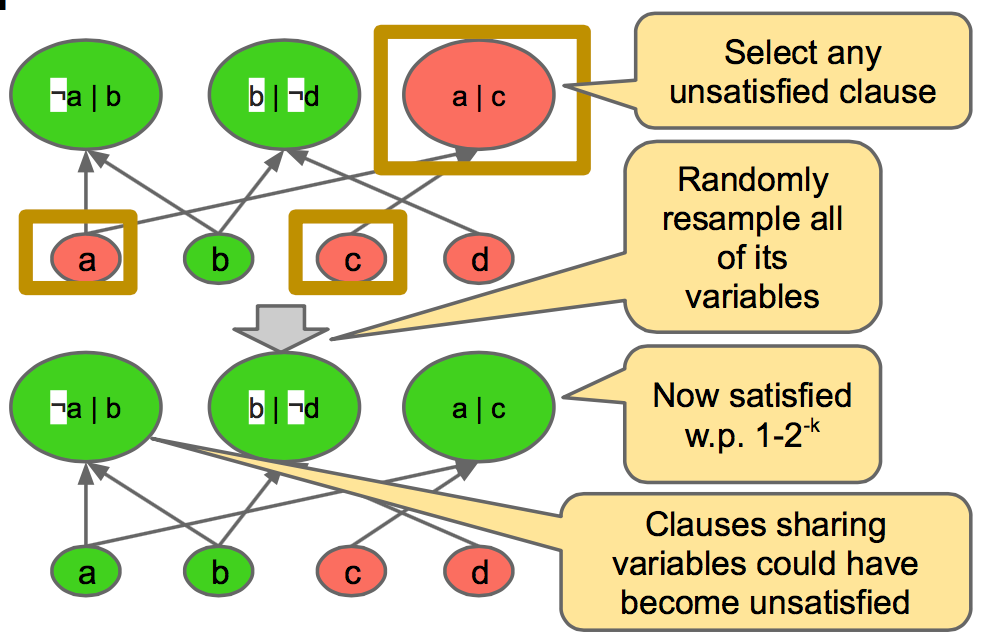
\includegraphics[scale=0.5]{figures/mt-directed-example.png}
    \caption{One iteration of an example run of the Moser-Tardos algorithm for \ksat.  The problem is to find an assignment to the binary variables $a$, $b$, $c$, and $d$ so that $(!a|b)\&(b|!d)\&(a|c)$.  The variables are initialized uniformly at random before the algorithm starts.}
    \label{fig:mt-directed-example}
  \end{mdframed}
\end{figure}

\begin{figure}[ht]
  \begin{mdframed}
    \centering
    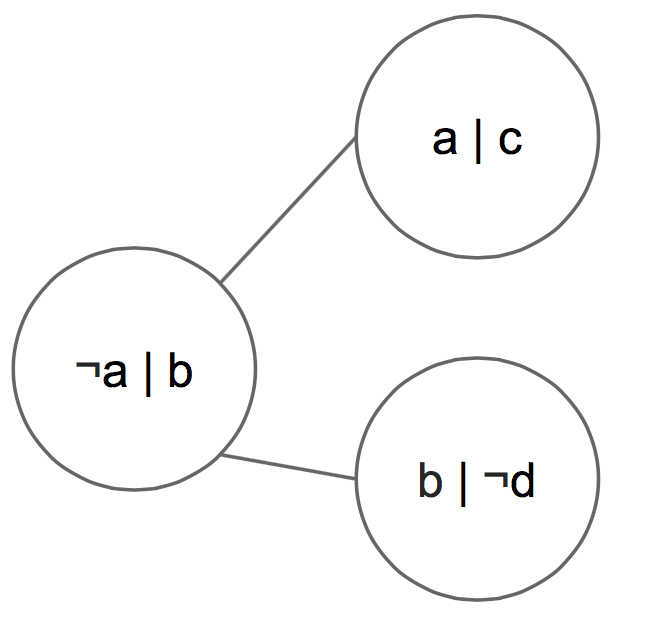
\includegraphics[scale=0.5]{figures/mt-undirected-example.png}
    \caption{The dependency graph for the problem pictured in figure \ref{fig:mt-directed-example}.  Here $d = 2$ and $p = 2^{-2}$, so the LLL condition $e p (d + 1)$ does not hold.}
    \label{fig:mt-undirected-example}
  \end{mdframed}
\end{figure}

Their proof uses a novel \emph{entropy compression} argument.  They show that the MT algorithm must terminate in a certain number of steps (on average) or it would be possible to represent the algorithm's state trajectory using fewer random bits than were used to generate it, which is impossible.  Tao \cite{tao2009entropy} and Fortnow \cite{fortnow2009entropy} make this argument more explicit.  Notice that taking $\mu$ to be the uniform distribution maximizes the entropy created at each step of the algorithm (at least on finite spaces), so it is easiest to make an entropy compression argument in that case.

After the Moser and Tardos paper, interest in the subject has only increased; follow-up work has given new algorithms, new problem domains, new applications, and a range of sufficient conditions weaker than the LLL condition.  Our interest, and the subject of this paper, is in strengthening the Moser-Tardos result from the \emph{variable} version of the problem to more general versions, under analogous conditions.  The key proof idea is taking the entropy compression argument seriously. %FIXME: Language.  Sounds arrogant.

\subsection{This paper}
In this paper, we first review the result by Moser and Tardos, using the more illuminating proof by Tao \cite{tao2009entropy} and Fortnow \cite{fortnow2009entropy} that directly highlights the role of entropy compression.  In section \ref{sec:perfect}, we review an extension of the algorithmic LLL to non-variable problems by Achlioptas and Iliopoulos \cite{achlioptas2014random}.  Achlioptas and Iliopoulos give a general condition on \emph{algorithms} rather than problems, and bring us partway to a general constructive LLL, but they require that the space $\Omega$ is finite, and this is the restriction we will remove.  In section \ref{sec:nonatomic-intro} we suggest that the entropy compression argument could be fruitfully extended to novel LLL-like applications in which the state vector of an algorithm cannot be uniquely recovered.  Achlioptas and Iliopoulos call such algorithms (or, technically, their associated random walk graphs) ``non-atomic''.  By removing the atomicity assumption, we can develop a more general constructive LLL. In section \ref{sec:examples} we give a series of motivating examples.  In section \ref{sec:markov}, we discuss an interpretation of the entropy compression argument as a statement about Markov chains and associated hidden Markov chains.  Finally, in section \ref{sec:nonatomic}, we give formal proofs.
%FIXME: Not clear this is a good organization.

\section{The algorithmic LLL}
\label{sec:lll}
Though the iterative version of the MT algorithm is very simple, a slightly more complicated \emph{recursive} one is useful for analysis:

\begin{algorithm}[H]
\caption{A more complicated recursive version of the Moser-Tardos (MT) algorithm.  This version replaces the \emph{arbitrary} order of resampling in algorithm \ref{alg:mt} with a fixed order that resamples neighborhoods of events in the dependency graph.}
\label{alg:mt-recursive}
\begin{algorithmic}
\Function{Solve}{$\mathcal{P}$, $\mathcal{A}$}
  \State Initialize $X \hasDist \mu$.
  \ForAll{$i \in [m]$}
    \Call{Fix}{i}
  \EndFor
  \Return $X$
\EndFunction

\Function{Fix}{i}
  \If{$! A_i(X)$}
    \Return
  \EndIf
  \State \Call{Resample}{i}
  \ForAll{$k \in [m] \texttt{s.t.} k \in \Gamma^{+}(i) \texttt{ and } A_k(X) = 1$}
    \Call{Fix}{j}
  \EndFor
\EndFunction

\Function{Resample}{i}
  \State Resample each $X_j \in \operatorname{vbl}(A_i) \hasDist \mu_j$.
\EndFunction

\end{algorithmic}
\end{algorithm}

An an introduction to later parts of this paper, we will give a proof that this algorithm terminates in polynomial time when the LLL condition is met.  Our argument mostly follows one by Tao \cite{tao2009entropy} and Fortnow \cite{fortnow2009entropy} that emphasizes the entropy compression aspect of the proof.  The argument is specialized to \ksat to make the exposition simpler, but we will later discuss the generalization to arbitary LLL problems.  We will prove that the specialization of algorithm \ref{alg:mt-recursive} to \ksat terminates before $m/2$ calls to \texttt{Resample}. %FIXME: Might be extra O(1) terms.
Recall that in the specialization to \ksat, $\mu$ is the uniform distribution on $\{0,1\}^n$-vectors and $A_i(X) = 1$ if clause $C_i$ is false.

%FIXME: This could do with division into subsections, since it is so long.

\subsection{A nice property of algorithm \ref{alg:mt-recursive}}
First, algorithm \ref{alg:mt-recursive} has a nice property that the simpler algorithm \ref{alg:mt} does not have, which motivates our switch to the more complicated version.  If \texttt{Fix}$(i)$ returns, $X$ cannot have flaw $A_i$, nor can it have any flaw it did not have before \texttt{Fix}$(i)$ was called.  The proof is by induction on the tree of calls to \texttt{Resample} caused by calling \texttt{Fix}$(i)$, which we (following Moser and Tardos) call a ``witness tree.''  In the witness tree (which we will be important later), each node is labeled (possibly nonuniquely) with a flaw index.  A call to \texttt{Fix}$(i)$ may cause a call to \texttt{Resample}$(i)$ and zero or more additional calls to \texttt{Fix} in the following loop.  There is a node in the tree for the call to \texttt{Resample}$(i)$, and that node has a child for each call to \texttt{Resample} caused by the calls to \texttt{Fix} in the loop.
%FIXME: Picture

The inductive argument is fairly simple.  If the tree is empty, then $X$ must not have flaw $A_i$, and no resampling occurred, so no additional flaws are added.  Otherwise, the variables $\operatorname{vbl}(A_i)$ were resampled and then calls to \texttt{Fix} were made for elements of clause $A_i$'s inclusive neighborhood (including $A_i$ itself) that were unsatisfied.  No other clauses could have become unsatisfied by this resampling, since clauses outside $\Gamma^{+}(i)$ do not have variables $\operatorname{vbl}(A_i)$.  By induction, these calls to \texttt{Fix} add no new flaws and satisfy each clause in $\Gamma^{+}(i)$.  So our call to \texttt{Fix}$(i)$ added no new flaws and ensured that $A_i$ was satisfied.
%FIXME: A little loose with the A_i and C_i notation here.
%FIXME: Should merge the witness tree description here, or break it into its own section.

This property implies that \ref{alg:mt-recursive} finds a satisfying solution if \texttt{Solve} returns at all, since it loops over all flaws and fixes each without introducing any new ones.  So it remains to show when (and how quickly) that happens.

We should emphasize that this fact is only \emph{convenient}, not necessary, for the following proof.  Algorithm \ref{alg:mt} enjoys many of the same guarantees as algorithm \ref{alg:mt-recursive}.

\subsection{The entropy compression argument}
The idea is to imagine running algorithm \ref{alg:mt-recursive} until \texttt{Resample} is called $t$ times.  We will give a scheme for compressing random bits -- which is impossible -- if $t$ is too large in expectation.  Let $\sigma_s$ denote the value of $X$ at the beginning of the $s$th call to \texttt{Resample}, and let $i(s)$ denote the argument to \texttt{Resample} on that iteration.  We will say that $A_{i(s)}$ was ``addressed'' on iteration $s$.  After $t$ calls, $\sum_{j = 1}^{t} \operatorname{vbl}(A_{t(j)}) = k t$ binary variables have been resampled independently using some random source.  The initial assignment used $n$ bits.  Let $Z \in \Omega^{t+1} = (\sigma_0, \sigma_1, \cdots, \sigma_t)$ denote the algorithm state vector.  Then $Z$ encodes $n + k t$ purely random bits.  We will use the assumption $2^C_0 p (d+1) < 1$ to give a method to encode the algorithm state in an alternative way $Y$, which we call the ``alternative information''.  (We will use $C_0 = 2$ and later $C_0 = \log_2 \frac{1}{0.3383}$, though the tightest constant is $C_0 = \log_2 e$.)  When $t$ is large on average, $Y$ will contain fewer bits than $Z$ on average.  That contradicts Shannon's source coding theorem \cite{shannon2001mathematical}, which formalizes the intuitive fact that it is impossible to encode purely random bits with a scheme that uses fewer bits in expectation.

We note first that, given an innocuous assumption about the problem (which is true for \ksat and can be made true for other problems), there is a 1-to-1 correspondence between the pair $((A_{t(i)})_{i=1}^{t}, \sigma_{t})$ and $Z$.  In other words, we assume that if we know the final return value and the sequence of flaws that were addressed, we know the whole sequence of states the algorithm passed through.  The assumption we need is that each flaw $A_i$ happens for only one setting of $\operatorname{vbl}(A_i)$.  For example, in \ksat, a disjunctive clause can only be violated by one setting of its variables.  In section \ref{subsec:trivial} we will explain why this assumption is innocuous in general.  Under the assumption, there is an easy inductive argument: If $\sigma_{i+1}$ and $A_{t(i)}$ are known, then $\sigma_i$ must equal $\sigma_{i+1}$ outside $\operatorname{vbl}(A_{t(i)})$, and on $\operatorname{vbl}(A_{t(i)})$ it must equal the one violating setting, since it was chosen to be \texttt{Resample}d.  But $\sigma_{t+1}$ and all the flaws are known, so the whole state vector $Z$ (including the initial state) is determined.
%FIXME: Include a picture.

It remains to encode $(A_{t(i)})_{i=1}^{t}$ efficiently.  Note that we cannot simply encode the addressed flaws using the natural encoding that takes $\log m$ bits, since this would lead us a different, much stronger condition than the LLL condition.  Instead we will use a structure called (by Moser and Tardos) a ``witness forest'' to hold instances in which flaws are addressed.  In this forest, there are two kinds of nodes:
\begin{description}
  \item[Roots:] Whenever the outer loop of the algorithm calls \texttt{Resample}$(i)$ and flaw $A_i$ currently happens, that flaw's variables are resampled, and then its neighbors in the dependency graph are potentially addressed.  We designate such outer-loop flaw-addressing instances as roots in the witness forest.  (When \texttt{Fix}$(i)$ is called but flaw $A_i$ does not currently happen, we add nothing to the forest.)
  \item[Children:] Whenever the inner loop in \texttt{Fix}$(i)$ calls \texttt{Fix}$(j)$, there must already be a node in the tree (either a root or, inductively, a child) corresponding to that flaw-addressing instance for flaw $i$.  When such a call results in a call to \texttt{Resample}$(j)$, we add a child to that node corresponding to flaw $A_j$.
\end{description}

For \ksat, $p = 2^{-k}$, since only one of the $2^k$ assignments to a disjunctive clause can violate it.  The assumption $2^C_0 p (d+1) < 1$ means that each flaw is independent of all but at most $2^{k-C_0}$ flaws, including itself.  So if an flaw-addressing instance is a child in the witness forest, it can be encoded using only $k-C_0$ bits.  This is the crux of the argument.  Unfortunately, things are slightly more complicated than that, because we must also encode the structure of the forest itself.  Encoding the identities and order of the roots is easy enough, since each flaw can appear at most once, and the order is by flaw index.  But encoding the individual trees is harder.  Given a complete graph on $t$ nodes, there are $t^{t-2}$ distinct spanning trees, so it takes $(t-2) \log_2 t$ bits to encode such trees \cite{prufer1918neuer,neville1953codifying}.  Since we also need to know the order of calls in the inner loop, and we can have potentially $m$ disjoint trees, the encoding length of a witness forest appears to be even greater than this.  If this were true, the average encoding length of a node would eventually become larger than $k$, ruining the proof.

However, we actually only need to encode the \emph{unlabelled structure} of each tree in the witness forest, and this is easier.  There is a simple encoding scheme, but let us add some intuition.  First, note that recording the order of calls in the inner loop is unnecessary, since the calls are made in a fixed order by flaw identity.  So if we are told only the identity of the root of each tree in the forest and the set of children of each node, we can reconstruct the order of each child set.  %FIXME: This is a bad explanation.  Needs pictures.
Second, we do not actually need to label the nodes of the tree.  We can just store the $k-C_0$-bit child identifiers in a some fixed order, for example the order in which a DFS visits nodes of the tree when children are ordered by their indices. %FIXME: Also needs a picture.
So the number of distinct witness trees to encode (ignoring the issue of encoding the roots, which we have already) is at most the number of \emph{unlabelled rooted trees} on $t$ nodes, which is much smaller than the number of labelled trees.  While there is no known exact formula for counting such trees, Otter \cite{otter1948number} gives an asymptotic estimate of
\seqn
  |\{T: T\texttt{ is an unlabelled tree}, |T| = n\}| \tilde O(1) (\frac{1}{0.3382\cdots})^t + O(1) .
\eeqn
Therefore (by Shannon's noisy channel coding theorem) there exists an encoding scheme for witness trees that uses only, say, $(\log_2 \frac{1}{0.3383}) t + O(1)$ bits.  Note that $\log_2 \frac{1}{0.3383}$ is only an upper bound on the number of required bits per iteration of the algorithm, since it assumes the maximum-entropy (uniform) distribution on unlabelled trees of size $n$, while the algorithm may generate witness trees with less entropy than that.

If we are willing to weaken the upper bound a bit, there is a very simple concrete encoding scheme that follows the algorithm execution.  First, we record the $k-C_0$-bit flaw data in the order in which \texttt{Resample} was called.  Then we record the history of the depth-first search executed in each tree by logging a $0$ whenever \texttt{Fix} is called inside \texttt{Fix}, and a $1$ whenever a call to \texttt{Fix} returns.  This uses at most $2$ bits per edge in the witness trees, thus at most $2t$ total bits.

So we can encode $Y$ using at most $n + m + (k - C_0 + 2)t$ bits, and we can determine $Z$ from $Y$, so by Shannon's source coding theorem
\seqn
  n + m + (k - C_0 + 2)t \leq n + k t \label{eqn:ksat-entropy-inequality}.
\eeqn

This is violated if $t \geq \frac{m}{C_0 - 2}$, so the algorithm must finish (in expectation) before that many iterations.  We have also shown that the algorithm must finish in expectation before $\frac{m}{C_0 - \log_2 \frac{1}{0.3383}} + O(1)$ iterations.  Moser and Tardos give a more careful argument considering the witness tree explicitly as a draw from a particular Galton-Watson process, bringing $C_0$ down to $\log_2 e$.  (This implies that the witness trees generated by algorithm \ref{alg:mt-recursive} are not uniformly distributed on the possible trees of fixed size.)

\subsection{Arbitrary starting state}
\label{subsec:arbitrary}
Note also that a similar proof would still work, with a worse bound, if we eliminated the requirement that the algorithm started in a uniform random state.  If the starting state is arbitrary, then it may have entropy $0$, and inequality \ref{eqn:ksat-entropy-inequality} would become
\seqn
  n + m + (k - C_0 + 2)t &\leq k t \\
  \implies t \leq \frac{n+m}{C_0-2} .
\eeqn
So we pay an additive penalty (at least according to this upper bound) equal to the dimension of the problem.  More generally, we pay a cost of $\log_2 |\Omega|$ when $\Omega$ is finite.  We will see this later when we review \cite{achlioptas2014random}.
%FIXME: Explain this better.
%FIXME: Forward-reference the section where we discuss this.

\subsection{General LLL problems}
\label{subsec:general-lll}
The proof above was restricted to \ksat.  In this subsection we outline the proof of the constructive LLL in full generality.

The important difference between \ksat and general LLL problems is that \ksat events are \emph{elementary}: For every flaw $A_i$, only a single assignment to the variables in $\operatorname{vbl}(A_i)$ causes $A_i$ to happen.  This allowed us to reconstruct the algorithm state vector $Y$ given only the final state $\sigma_{t}$ and the vector of flaws addressed $(A_1, \cdots, A_t)$.  Each flaw could be addressed using $\log_2 (d+1) + C_0$ bits, but from its identity we reconstructed one out of $2^k$ possible assignments, $k = \log_2 2^k = \log_2 (1/p)$ bits of information.  The contradiction arose because $\log_2 (1/p) > \log_2 (d+1) + C_0$, which is exactly the LLL condition.

Now that we have stated the argument in this way, the general case is straightforward.  Assume that we know $\sigma_{i+1}$ and $A_i$.  Then we know that $\operatorname{vbl}(A_i)$ take values in $\sigma_i$ with joint probability at most $p$.  If $\Omega$ is discrete, then we have gained $\log_2 (1/p)$ bits of information about $\sigma_i$.  If we used only $\log_2 (d+1) + C_0$ bits to encode it, we eventually get the same contradiction.

If $\Omega$ is continuous, then the same is true, except that we must make our arguments in terms of an abstract differential entropy rather than bits.  We have also ignored the fact that our argument was inductive, and when there is some uncertainty remaining in $\sigma_{i}$, we no longer know it exactly when we try to infer $\sigma_{i-1}$.  Both issues are surmountable, but we will defer that to section \ref{subsec:trivial}.

\subsection{The simple Moser-Tardos algorithm}
Algorithm \ref{alg:mt-recursive} is convenient for analysis, but algorithm \ref{alg:mt} is easier to describe and implement, and it leads to parallel algorithms.  In this subsection we outline the proof of the constructive LLL with algorithm \ref{alg:mt}.
%FIXME

\subsection{A weaker condition}
Moser and Tardos actually prove that their algorithm terminates successfully in polynomial time under a weaker condition than $e p (d+1) < 1$.  Under some assignment of a weight to each flaw $x: \mathcal{A} \to (0,1)$, the following condition must hold for every flaw $A_i$:
\seqn
  P(A_i) \leq x(A_i) \prod_{j \in \Gamma(i)} (1-x(A_j)) (\forall A_i \in \mathcal{A}) \label{eqn:general-lll-req}
\eeqn

This condition is more complicated and unnecessary for exposition, so we have  focused mostly on the simpler one.  However, it is often the condition cited in the literature, so it is important to see the connection between the two conditions.  Let us briefly show that $e p (d+1) < 1$ implies the weaker condition with $x(A_i) = \frac{1}{d+1}$ for all $i$.  $P(A_i) \leq p$ for all $i$ by definition of $p$, so the (claimed) stronger condition gives us:
\seqn
  P(A_i) \leq p &< \frac{1}{d+1} \frac{1}{e}  \\
  &< \frac{1}{d+1} (1 - \frac{1}{d+1})^d \\
  &\leq \frac{1}{d+1} \prod_{j \in \Gamma(i)} (1-\frac{1}{d+1}) \\
  &= x(A_i) \prod_{j \in \Gamma(i)} (1 - x(A_j)) .
\eeqn

The proof of the constructive LLL under condition \ref{eqn:general-lll-req} uses the condition to construct a Galton-Watson process whose entropy lower-bounds that of the witness trees actually generated by algorithm \ref{alg:mt-recursive}.  Moser and Tardos do not use the word ``entropy'' explicitly anywhere in their paper.  Instead, they bound the probability of any tree appearing with a particular root and sum those probabilities over trees and roots to bound the expected number of elements of a witness tree.  It would be interesting to give a version of the proof that more explicitly relies on the entropy compression argument, but we will not do that here.
%FIXME

\section{The algorithmic LLL on general sample spaces}
\label{sec:perfect}
Thus far, we have seen only a variable-version LLL problem in which our probability space was a product of $n$ variables.  The MT algorithm requires explicit access to those variables, and it is restricted to handling every flaw in the same way -- by resampling all of its variables from the projection of $\mu$ on the lower-dimensional space of those variables.  Both assumptions are satisfied for many interesting problems, but it is still useful to see how they can be relaxed.  The sample space for some combinatorial problems is better represented in other forms, such as permutations \cite{achlioptas2014random} or more generally random injections \cite{lu2007injections}.  And contra the second assumption, many local search algorithms for \ksat (e.g. \texttt{WalkSAT} \cite{papadimitriou1991selecting}) are similar to MT, but will flip only a smaller number of variables on each iteration, and with a more complicated random component.
%FIXME: These are weak examples.
The proof of Moser and Tardos assumes a \emph{particular} search algorithm and applies to a \emph{somewhat broad} class of problems, but it would be nice to have a way to prove efficiency of a broader class of algorithms (and perhaps for an even broader class of problems).  Achlioptas and Iliopoulos \cite{achlioptas2014random} take a step in this direction, providing an elegant framework for proving efficiency of random local search algorithms in arbitrary finite spaces.  Examining this framework is instructive.

Again take our $\sigma$-algebra to be $(\Omega, \Sigma)$, but this time without a product structure and without even a measure $\mu$.  Our set of flaws is the same as before, but now there can be no notion of $\operatorname{vbl}(A_i)$.  Let $U(\sigma)$ denote the set of flaws that happen under state $\sigma$.  Again, our goal is to find a flawless element $\sigma^* \in \Omega$.  Consider any randomized iterative algorithm whose random state is Markovian and stationary, which attempts to find a flawless object.  (The MT algorithm is an example of such an algorithm.)  By definition, we can view any such algorithm as a random walk $\mathcal{T}$ on a graph whose nodes are $\Omega$ and whose edge-weights define a transition matrix for the walk.

%The argument in section \ref{sec:lll} was really an argument about %FIXME
Now let us try to write down the properties of these graphs that are really needed for something like the proof in section \ref{sec:lll} to apply.

The first requirement is ``atomicity,'' which generalizes Moser's and Tardos' concept of ``elementary'' flaws in section \ref{subsec:general-lll}.  We needed the fact that the flaw $A_s$ addressed on iteration $s$ uniquely determined the values of $\operatorname{vbl}(A_s)$ in the previous state $\sigma_s$.  We proved this by assuming, by induction, that we knew the values of the variables in $\sigma_{s+1}$.  Given the identity of the flaw, we knew that $\sigma_s$ and $\sigma_{s+1}$ differed only on the variables in $\operatorname{vbl}(A_s)$ differed.  Further, since each flaw could be violated by only one configuration of its variables, we knew what that configuration must have been in $\sigma_s$.  Without variables, we need a different tack to get a correspondence between flaw vectors and algorithm state vectors.  We will still assume that the algorithm ``addresses'' a single flaw on each iteration; given a current state $\sigma_t$ and a flaw to address, the algorithm draws from some distribution to find its next action.  (The transition probabilities for each node are obtained by marginalizing out the flaw selection distribution.)  To achieve accountability, we assume that, for every (flaw, state) pair $(A_{s}, \sigma_{s+1})$, there is a unique previous state $\sigma_s$.  In terms of the random walk graph, this means that if we label each weighted edge in the graph with the flaw we addressed at that step, each node has at most one incoming edge for each flaw.  This property is called atomicity.

In the variable version of the problem, there are two simple sufficient conditions for atomicity:
\begin{description}
  \item[Simple constraints:] For each flaw $A_i$, there is only one configuration of the variables $\operatorname{vbl}(A_i)$ that makes the flaw happen.  This condition is unimportant, since we can always modify the algorithm (for purposes of proofs) to make it so.  We will discuss this further in section \ref{subsec:trivial}.
  \item[Algorithmic focusing:] After choosing a flaw $A_s$, the algorithm modifies \emph{only} the variables in $\operatorname{vbl}(A_s)$ on iteration $s$.  This condition is nontrivial.
\end{description}

The second requirement is analogous to the standard LLL condition $e p (d+1)$ (though other, more elaborate results are proven in \cite{achlioptas2014random}).  In section \ref{sec:lll}, we saw that it was desirable (from the perspective of the entropy compression argument) to maximize the entropy of each step.  So we will assume that, having chosen a flaw $A_s$ to address, our algorithm chooses uniformly at random from all the possible next states it could reach.  We call this ``action set'' $A(A_s, \sigma_s)$.  (In the variable version with binary variables, this would have been of size $2^{\operatorname{vbl}(A_s)}$ for any $\sigma_s$.)  Then, the requirement is that no flaw $A_i$ has too many neighbors with small action sets; specifically,
\seqn
  \label{eqn:degree-req}
  e \sum_{j \in \Gamma(i)} \frac{1}{\min_{\sigma: A_j \in U(\sigma)} |A(\sigma, A_j)|} < 1 - \delta
\eeqn
for some positive $\delta$.
%FIXME: Rephrase the previous results in terms of \delta; this language is clearer.
%FIXME: Note that A-I have the uniformity assumption, which we could relax later.

Under these two requirements, Achlioptas and Iliopoulos show that any such algorithm will terminate quickly.  The running time of the random walk algorithm is $\delta^{-1} (\log_2 |\Omega| + |U(\sigma_1)| + s)$ steps with probability at least $1 - 2^{-s}$.  Though this is a high-probability bound rather than a bound in expectation, it is similar to the running time we found in section \ref{sec:lll}.  Here $|U(\sigma_1)|$, the number of flaws in the initial assignment, stands in for $m$, which we used to upper-bound the same quantity in section \ref{sec:lll}.  The $\log_2 |\Omega|$ term is introduced because Achlioptas and Iliopoulos assume an arbitrary starting location; we found the same additive constant in section \ref{subsec:arbitrary}.  And $\delta^{-1}$ is a slack term analogous to $C_0 - 2$.
%FIXME: When we rephrase the above stuff in terms of \delta there will be a direct correspondence.
The main point of our interest in \cite{achlioptas2014random} is the clear statement of the atomicity requirement, and we will not revise their proof.  Note that, by working directly with the random walk graph and paying the extra $\log_2 |\Omega|$ cost in running time, Achlioptas and Iliopoulos avoid assuming a measure $\mu$ on $(\Omega, \Sigma)$.  We will have to reintroduce the measure when we attempt to generalize their result to infinite spaces.  This seems to be a very mild restriction.

\section{Non-atomic algorithms}
\label{sec:nonatomic-intro}
In sections \ref{sec:lll} and \ref{sec:perfect}, we saw that the \emph{atomicity} of an \mt algorithm was a key assumption in the entropy-compression argument.  In this section, we show that similar arguments can be made without the atomicity assumption.  This raises the possibility of using the algorithmic LLL in applications outside combinatorial search.

Recall that assumptions on the degree of nodes in the transformation graph of an \mt algorithm allowed us to show that the identity of the flaw addressed at each step could be encoded using fewer bits on average than would be needed to encode the randomness involved in making the step itself.  Assuming atomicity (recall its two requirements: (1) simple constraints and (2) algorithmic focusing) then gave us a way to exactly reconstruct the state of the algorithm before the step was taken.  Now, let us abstractly write $Z$ for a vector of algorithm states (in the MT algorithm for \ksat, the concatenation of the original uniform assignment bits and the vectors of $k$ bits used at each iteration); $Y$ for the hypothetical observed information that encodes information sufficient to reconstruct the algorithm states (in our explication of Tao's MT proof, this includes the witness forest, the set of flaws of the initial assignment, and the final assignment); and $\operatorname{Infer}$ for the deterministic function that maps $Y$ to $Z$.  Write $P(Z | Y)$ for the posterior distribution (after Bayesian updating) on the true algorithm state vector given the alternative information.  The purpose of the atomicity assumption is that $P(Z | Y)$ is a point mass measure at $\operatorname{Infer}(Y)$.

Existing work, including \cite{achlioptas2014random}, assumes that it is necessary for $P(Z | Y)$ to be a point mass, but what would it mean if it were not?  We could recast the original entropy compression argument as a \emph{relative entropy compression} argument.

Consider the state vector for $t$ steps of the \mt algorithm for \ksat, which is of size $M = m + kt$.  Then the ``prior'' on $Z$, the distribution before we observe anything, is $P(Z) = \operatorname{Unif}(2^{m+kt})$.  By Bayes' rule, 
\seqn
  \label{eqn:entropy-general}
  H(Z) = H(Z | Y) + H(Y) - H(Y | Z) .
\eeqn

Typically we will proceed by finding a simple expression or lower bound for the left hand side (which is typically determined explicitly by the algorithm) and upper-bounding the right hand side.  Since entropies are nonnegative, we can simply drop the $H(Y | Z)$ term when searching for an upper bound, if it is convenient.  And if, for example, we can encode the alternative information $Y$ using $\hat{H}(Y)$ bits, an upper bound on the prior entropy $H(Y)$ is $\hat{H}(Y)$, and then equation \ref{eqn:entropy-general} becomes
\seqn
  \label{eqn:entropy-encoded}
  H(Z) \leq H(Z | Y) + N .
\eeqn
(Note that we need $\operatorname{Unif}(\{0,1\}^d)$ to be a suitable base measure for computing or bounding $H(Z)$ and $H(Z | Y)$.)  When $P(Z | Y)$ is a point mass, $H(Z | Y) = 0$, and inequality \ref{eqn:entropy-encoded} reduces to
\seqn
  \label{eqn:entropy-tao}
  H(Z) \leq N .
\eeqn
This is exactly the fact that we needed in section \ref{sec:lll} to show a contradiction when $t$ was too large, having shown that both $H(Z)$ and $N$ were affine functions of $t$.

From this perspective, it does not seem strictly necessary that $H(Z | Y) = 0$ or that $Y$ and $Z$ be representable by finitely many bits.  Perhaps in some cases we can use inequality \ref{eqn:entropy-encoded} or equation \ref{eqn:entropy-general} with some other upper bounds on $H(Z | Y)$ or $H(Z)$ to make an entropy compression argument.  We will consider several examples to illustrate this point.

\section{Examples}
\label{sec:examples}
\subsection{Example 1 (trivial)}
\label{subsec:trivial}
As a trivial example, suppose that we have run the MT algorithm for a \ksat problem and encoded the alternative information in $Y$ using a bit string of size at most $h$ for each iteration, as in Tao's proof.  Imagine removing one bit of information from each iteration's bit string in such a way that we can infer from it only a uniform distribution over $2^c$ potential flaws; call this reduced alternative information $Y'$, with encoding length $N' = N - ct$.  This ensures there are $2^{ct}$ possible flaw-encodings, and thus (by atomicity of the underlying MT algorithm for \ksat) our posterior on $Z$, having observed $Y'$, is a uniform distribution over $2^{ct}$ state vectors.  Then we could use Tao's argument to show that inequality \ref{eqn:entropy-encoded} is violated under exactly the conditions when it was violated for $Y$, since $H(Z | Y') + N' = H(Z | Y) + ct + N - ct = H(Z | Y) + N$.

We can use exactly the same argument to apply Tao's proof in a situation where the ambiguity in $P(Z | Y)$ is induced by non-atomicity of the transformation graph, rather than by the artificial removal of information from $Y$.  If $c$ states can lead to a single state by addressing the same flaw, then we now require that $e c p (d + 1) < 1$.
%FIXME

So why do we call this example trivial?  It only violates the first condition for atomicity in the framework of Achlioptas and Iliopoulos, which is that if we observe state $\sigma_{t+1}$ after a flaw $f$ is addressed, there is only one possibility for the previous state $\sigma_t$.  They call this condition ``syntactic,'' since it can always be addressed (when $\Omega$ is finite) by expanding the flaw set to make flaws more granular.  For example, say that we have a modified version of \ksat in which $2^c$ out of $2^k$ assignments to each clause can make it fail.  We can rephrase any such problem as an abstract \ksat-like problem by making $2^c$ copies of each clause, with each copy only disallowing one state.  This would increase the size of $\mathcal{A}$ by $2^c$ and increase by $c$ the number of bits required to describe any flaw in the alternative information.  (In terms of the conditions in Achlioptas' and Iliopoulos' work, the number of %FIXME
So the argument in our trivial example does not buy us any extra power in handling non-atomicity, only an alternative proof of Achlioptas' and Iliopoulos' comment.  And in the framework of Moser and Tardos, it buys us nothing, since they do not require atomicity, but rather a bound $p$ on the marginal probability of flaws.

\subsection{Example 2 (Uncountable feasible set)}
\label{subsec:uncountable}
Now let us see an example of a problem and algorithm that are covered by the Moser-Tardos framework under some burdensome assumptions.  Consider the following feasibility problem:
\seqn
  \label{prob:feas}
  \operatorname{Find} & x \in \Reals^n \texttt{s.t.} \\
  A_i(x) = 0 \forall i \in [m] ,
\eeqn
where the $A_i$ are indicator functions $\Reals^{m} \to \{0,1\}$.

We can write down an MT algorithm to solve this problem.  This will add some assumptions, two of which we must discuss before even writing down the algorithm.  First, we assume that each function depends only on a subset of the elements of the vector $x$; let $\operatorname{vbl}(f) \subseteq [n]$ denote the indices on which a function $f$ depends, and let $y[\operatorname{vbl}(f)]$ denote the corresponding elements of a vector $y$.  Second, we must write down a \emph{measure} $\mu = \prod_{j=1}^{n} \mu_j$ on $\Reals^n$, where each $\mu_j$ is a measure on $\Reals$.  During the algorithm, we must be able to sample from $\mu$ and from product measures of the form $\prod_{j \in \operatorname{vbl}(A_i)} \mu_j$.  Later we will have to impose additional constraints on $\mu$, but for now imagine that $\mu_j = N(0, 1)$ for each $j$.

\begin{algorithm}[H]
\caption{An MT-like algorithm for problem \ref{prob:feas}.}
\label{alg:mt-feas}
\begin{algorithmic}[1]

\State Initialize $x \hasDist \mu$.
\ForAll{$i \in [m]$}
  \Call{Fix}{i}
\EndFor

\Function{Fix}{i}
  \If{$A_i(x) = 0$}
    \Return
  \EndIf
  \State Resample $x[\operatorname{vbl}(A_i)]$ from $\prod_{j \in \operatorname{vbl}(A_i)} \mu_j$.
  \ForAll{$k \in [m]: k \in \Gamma(i), A_k(x) = 1$}
    \Call{Fix}{$k$}
  \EndFor
\EndFunction

\end{algorithmic}
\end{algorithm}

Moser and Tardos prove that this algorithm finishes in polynomial time under the following conditions:

\begin{enumerate}
  \item $n$ is finite. \label{eqn:feas-finitedim-condition}
  \item Each $A_i$ is $\mu$-measurable and satisfies $\mu(\{x: A_i(x) = 1\}) \leq p$ for some small $p$.  That is, random sampling from our measure $\mu$ satisfies each single constraint with high probability.  (The difficulty of the problem comes from the requirement of satisfying the constraints \emph{jointly}.)  Otherwise the constraints can be arbitrarily complicated.  \label{eqn:feas-margprob-condition}
  \item $\mu$ is a product measure $\prod_{j=1}^{n} \mu_j$, where each $\mu_j$ is a measure on $\Reals$.  During the algorithm, we must be able to sample from $\mu$ and from product measures of the form $\prod_{j \in \operatorname{vbl}(A_i)} \mu_j$.  \label{eqn:feas-prodmeasure-condition}
  \item The dependency graph induced by the constraints and the measure $\mu$ meets the usual LLL condition: $e p (d+1) < 1$. \label{eqn:feas-lowdep-condition}
\end{enumerate}

% \begin{enumerate}
% %FIXME: Some of these comments are useful to have here.
%   \item We chose our sample space to be a norm ball in finite dimensions, rather than say all of $\Reals^n$, precisely so that our sample space would be compact, allowing us to choose a simple probability measure as our dominating measure when computing entropies.  In general, to bound the number of steps taking by the algorithm, we need a probability measure that $Y$-almost surely dominates $P(Z | Y)$, for which the LLL-required marginal flaw probabilities hold, and which induces low dependency degree among the flaws.
%   \item We chose the infinity norm ball in particular for a different reason: the sample space needs to be an axis-aligned rectangle, or it is not easy to ensure that the resampling step keeps us inside it while modifying only $k$ variables at a time and covering a large volume.  Again, this is not important for proving something about the number of steps taken by the algorithm, but it is important for the efficiency of the individual steps.
%   \item Rather than augment $Y$ to pin down $Z$, we could imagine proving directly that $H(Z | Y)$ is small.  It is natural to view $Z$ and $Y$ as the states and observations of a hidden Markov model, respectively, and use any of the well-known algorithms for inference in HMMs to compute $P(Z | Y)$.  (Such inference could be quite difficult if the constraint functions are complicated, but for purposes of analysis we could imagine performing it.)  At least in this case, augmenting $Y$ was much simpler, but this makes the example weaker, since we are not taking advantage of our freedom in making $H(Z | Y) > 0$.
%   \item With respect to the constraint functions themselves, the algorithm can be made efficient as long as we have an oracle that can efficiently find a violated constraint when there is one.  It may be possible to have an efficient version of the algorithm testing only a core of $\operatorname{poly}(n)$ ``core'' constraints using the ideas of Haeupler et al \cite{haeupler2011new}.
% \end{enumerate}

In our next example, we will remove the finite-dimensionality restriction.

\subsection{Example 3 (Infinite-dimensional feasible set)}

\label{subsec:infinitedim}
Now consider the following modified feasibility problem:
\seqn
  \label{prob:feas-infinitedim}
  \operatorname{Find} & x \in \Omega \\
  A_i(x) = 0 \forall A_i \in \mathcal{A} .
\eeqn
Again the $A_i$ are \emph{arbitrary} indicator functionals $\Omega \to \{0,1\}$, though now there may be infinitely many of them.
We assume $\Omega$ is a Hilbert space so that it admits a countable basis, and we endow it with a probability measure $\mu$.  (For example, we could be optimizing over functions on some underlying space, and $\mu$ could be a Gaussian process measure.)  Let $(\phi_j)_{j \in \Nats} \in \Omega^{\Nats}$ be a countable basis for $\Omega$, and let $\phi(x) = (\inprod{\phi_j}{x} \phi_j)_{j \in \Nats} \in \Omega^{\Nats}$ be the basis representation of an element $x \in \Omega$.  Again, we will assume that each constraint functional depends only on a subset of the elements of $\phi(x)$; let $\operatorname{vbl}(z) \subseteq \Nats$ denote the indices of basis elements on which a constraint functional $z$ depends, and let $\phi(y)[\operatorname{vbl}(z)]$ denote the corresponding elements of the basis representation of $y \in \Omega$.  Finally, for $A \subset \Nats$ a (possibly infinite) subset of indices for basis elements, and $a$ a vector of weights for those elements, let $P_{|B}(E | a)$ denote the conditional $\mu$-measure of event $E$ given the event $(\phi[A])^{-1}(a)$.  This generalizes the projections of product measures from which we resampled variable subsets in the finite example.  Having eliminated the assumption that $\mu$ is a product measure, this is a natural distribution for resampling.

We can write down an MT-\emph{like} algorithm for solving this problem:

\begin{algorithm}[H]
\caption{An MT-like algorithm for problem \ref{prob:feas-infinitedim}.}
\label{alg:mt-feas-infinitedim}
\begin{algorithmic}[1]

\State Initialize $x \hasDist \mu$.
\ForAll{$i \in [m]$}
  \Call{Fix}{i}
\EndFor

\Function{Fix}{i}
  \If{$A_i(x) = 0$}
    \Return
  \EndIf
  \State Resample $\phi(x)[\operatorname{vbl}(A_i)]$ from $P_{|\Nats \setminus \operatorname{vbl}(A_i)}(\cdot | \phi(x)[\Nats \setminus \operatorname{vbl}(A_i)])$.
  \ForAll{$j \in [m]: j \in \Gamma(i), A_j(x) = 1$}
    \Call{Fix}{j}
  \EndFor
\EndFunction

\end{algorithmic}
\end{algorithm}

Soon we will provide a proof that this algorithm finishes in expected polynomial time under conditions analogous to the LLL conditions.  Specifically, we will make the following assumptions:

%FIXME: No idea what these should be, really.
\begin{enumerate}
  \item Each $A_i$ is $\mu$-measurable.
  \item Further, each flaw must be addressed with positive probability when we resample it.  More precisely, there is an upper bound $p^* < 1$ on the probability of any single flaw happening when we resample conditional on the variables on which it does not depend, regardless of the value of those variables:
    \seqn
      \label{eqn:feas-condprob-condition}
      p^* = \sup_{A_i \in \mathcal{A}} \esssup_{x \in \Omega} P_{|\Nats \setminus \operatorname{vbl}(A_i)}(A_i | \phi(x)[\Nats \setminus \operatorname{vbl}(A_i)]) .
    \eeqn
    $p^*$ is analogous to $p$ in the standard LLL.
  \item The dependency graph induced by our constraints meets a slightly-strengthened version of the usual LLL condition: $2^{C_0} p^* (d+1) < 1$, for some absolute constant $C_0$.  (If $C_0 = \log_2 e$ then this result specializes to the standard LLL.) \label{eqn:feas-lowdep-strong-condition}
\end{enumerate}

% Some possible alternative conditions, from A-I paper:
% \begin{enumerate}
%   \item Each $A_i$ is $\mu$-measurable.
%   \item Further, each flaw must be addressed with positive probability when we resample it.  More precisely, there is a positive lower bound $p^*$ on the probability of each flaw not happening when we resample it conditional on the variables on which it does not depend, regardless of the value of those variables:
%     \seqn
%       \label{eqn:feas-margprob-condition}
%       p^* = \inf_{A_i \in \mathcal{A}} \essinf_{x \in \Omega} P_{|\Nats \setminus \operatorname{vbl}(A_i)}(\bar{A_i} | \phi(x)[\Nats \setminus \operatorname{vbl}(A_i)]) .
%     \eeqn
%     $p^*$ is analogous to $p$ in the standard LLL.
%   \item The dependency graph induced by our constraints meets a slightly-strengthened version of the usual LLL condition: $2^{C_0} p^* (d+1) < 1$, for some absolute constant $C_0$.  \label{eqn:feas-lowdep-condition}
% \end{enumerate}


%FIXME: Explain that this algorithm is not obviously implementable because the space is infinite-dimensional.  For now, could just cite some sources that use infinite-dimensional objects by representing them implicitly, and argue that this could be possible if the constraint functions behave that way.  Admit that we don't currently know of an application.

%
% This problem now has many of the ingredients of an LLL problem.  (In fact, we can encode any instance of \ksat that satisfies the LLL conditions in this problem, mapping $x_i$ to \texttt{true} if it is in $[0,1]$ and \texttt{false} otherwise, and encoding constraints accordingly.)  The process for encoding the alternative information and constructing a witness forest from it is almost identical to that in Tao's argument.  A technical difficulty is that the sample space is uncountable, so we can no longer speak of encoding a point using bits; this is where it is useful to use the entropy inequality \ref{eqn:entropy-general} directly.  A more practical difficulty is that we can no longer exactly reconstruct the algorithm state given the history of corrected flaws.  To fix this, it will suffice to augment the alternative information slightly.
%
% Let us first calculate $H(Z)$ for a run of algorithm \ref{alg:mt-feas} that takes $t$ steps.  This part is easy.  We define $Z$ to be the concatenation of the initial algorithm state (a draw from $\mu^n$) and the $t$ resampling steps (equivalent to draws from $\mu^k$).  When computing entropies, we use as our reference measure $\mu^n$.  Each of our events is independent, so $H(Z) = H(U([-1,1])) (n + t k) = n + k t$.
%
% Now we define the alternative information $Y$ and find an upper bound for its entropy $H(Y)$.  We use almost the same construction as in Tao's proof: $Y$ is the concatenation of
% \begin{enumerate}
%   \item the witness forest (a number of bits, whose entropy is therefore bounded by its length),
%   \item the end state (whose entropy is at most $n$, the same as that of the initial algorithm state),
%   \item the initial set of violated constraints (which uses at most $m$ bits), and
%   \item one additional piece of information for each iteration, which was not needed in Tao's argument.  To apply Tao's argument directly, we need to exactly reconstruct each state $\sigma_t$ from $Y$.  But at each iteration, even if we know $\sigma_{t+1}$ and the rest of $Y$ tells us exactly the flaw that has been addressed, we cannot in general exactly reconstruct the previous algorithm state $\sigma_t$.  However, we can bound its support, which bounds its entropy under the dominating measure $\mu^n$, and then include addition information in $Y$ sufficient to pin down $\sigma_t$ precisely.  Under our assumptions on the problem, it turns out that this additional data has entropy at most $1$.  Given only the values of $\sigma_t$ on the $n - k$ variables outside $\operatorname{vbl}(A_t)$, we know that $\mu^n(A_t | \{(\sigma_{t+1})_i: i \notin \operatorname{vbl}(A_t)\}) \leq 2^{-k}$, since $A_t$ is independent of those variables and $\mu(A_t) \leq 2^{-k}$ by assumption \ref{eqn:feas-margprob-condition}.  This happens inside a subset of size $2^{k}$, which has $\mu^n$-measure $2^{k-n}$, so the set of possible values for $\sigma_t$ is of $\mu^n$-measure $2^{-n}$, and its entropy (with $\mu^n$ as dominating measure) is $1$. %FIXME: Make the entropy argument more precise.  We are considering each item independently, which gives an upper bound, which is all we want.
% \end{enumerate}
%
% From these pieces and their individual entropy bounds (the sum of which bounds the joint entropy), $H(Y) \leq m + n + (k - C_0 + 2) t$, where $C_0$ is the constant in assumption \ref{eqn:feas-lowdep-condition}.
%
% Finally, since we have pinned down $Z$ using $Y$, $H(Z | Y) = 0$.  Putting everything together, we get $m + n + (k - C_0 + 2) t \leq n + k t$, so that the algorithm must terminate (in expectation) before $t > \frac{m}{C_0 - 2}$.  We can choose $C_0 = 3$, giving us the requirement that $8 p d < 1$.  The algorithm terminates only when no constraint is violated, so the algorithm must find a satisfying solution in $m$ calls to \texttt{Fix}.  (Note that the ordinary non-constructive LLL applies to this problem, and our assumptions are slightly stronger than the LLL conditions, so a solution must exist.)
%
% Some final notes on this algorithm:
% \begin{enumerate}
%   \item We chose our sample space to be a norm ball in finite dimensions, rather than say all of $\Reals^n$, precisely so that our sample space would be compact, allowing us to choose a simple probability measure as our dominating measure when computing entropies.  In general, to bound the number of steps taking by the algorithm, we need a probability measure that $Y$-almost surely dominates $P(Z | Y)$, for which the LLL-required marginal flaw probabilities hold, and which induces low dependency degree among the flaws.
%   \item We chose the infinity norm ball in particular for a different reason: the sample space needs to be an axis-aligned rectangle, or it is not easy to ensure that the resampling step keeps us inside it while modifying only $k$ variables at a time and covering a large volume.  Again, this is not important for proving something about the number of steps taken by the algorithm, but it is important for the efficiency of the individual steps.
%   \item Rather than augment $Y$ to pin down $Z$, we could imagine proving directly that $H(Z | Y)$ is small.  It is natural to view $Z$ and $Y$ as the states and observations of a hidden Markov model, respectively, and use any of the well-known algorithms for inference in HMMs to compute $P(Z | Y)$.  (Such inference could be quite difficult if the constraint functions are complicated, but for purposes of analysis we could imagine performing it.)  At least in this case, augmenting $Y$ was much simpler, but this makes the example weaker, since we are not taking advantage of our freedom in making $H(Z | Y) > 0$.
%   \item With respect to the constraint functions themselves, the algorithm can be made efficient as long as we have an oracle that can efficiently find a violated constraint when there is one.  It may be possible to have an efficient version of the algorithm testing only a core of $\operatorname{poly}(n)$ ``core'' constraints using the ideas of Haeupler et al \cite{haeupler2011new}.
% \end{enumerate}

%\subsection{Example 3 (An Unfocused Algorithm)}

\section{A non-ergodic Markov chain interpretation}
\label{sec:markov}
Our first step is to prove a general theorem about random walks.  Achlioptas and Iliopoulos discuss random walks that find perfect objects under two conditions:
\begin{enumerate}
  \item The random walk must be perfectly reconstructable given a perfect object and a tree-history of addressed flaws.
  \item The random walk must end up in a $0$-entropy state, which we can think of as either a terminating state or a self-loop with probability $1$.  These states, and only these states, must be our desired perfect objects.
\end{enumerate}
In this section, we generalize this notion to \emph{highly-reconstructable} random walks that hit \emph{low-transition-entropy subgraphs}.  This is reminiscent of the fact that a random walk will quickly find a subgraph of small conductance.

First, some setup and notation.  Fix a $\sigma$-algebra $(U, \Sigma)$.  A \emph{random walk graph} is a weighted digraph $G = (U, E, w)$ for which the edges leading out of each node define a probability distribution.  That is, $w(i, \cdot)$ is a probability measure on $U$ (perhaps supported only on a ``neighborhood'' of $i$) for all nodes $i$.  We define the edges and weights of a \emph{node-induced} random walk subgraph $G'$ of $G$ on nodes $U'$ as follows: $G'$ has nodes $U'$, edges $\{(i,j): (i,j) \in E; i, j \in U'\}$, and renormalized weights $w'(i, \cdot) = 1[i \in U'] 1_{U'} \frac{1}{w(i, U')} w(i, \cdot)$.  (We assume $w(i, U') > 0$ for all $i \in U'$.)
%FIXME: Kinda sloppy.  Do we need to allow U' to have measure 0 sometimes?
%FIXME: This repeats some of \ref{sec:perfect}.

Fix a (possibly infinite) random walk graph $G = (U, E, w)$ and a node-induced subgraph $G' = (V, F, w')$.  We will define $V$ later.  Think of $V$ as the set of flawed states and $\bar{V} = U \setminus V$ as the set of flawless states.

Let the stochastic process $\sigma(\mu, G) = (\sigma_0, \sigma_1, \cdots) \in U^\infty$ be the infinite Markov chain recording states of a random walk that starts by drawing $\sigma_0 \hasDist \mu$ and drawing $\sigma_{i+1} \hasDist w(\sigma_i, \cdot)$.  (When the graph and starting measure are clear we will just write $\sigma$.)  And let $\sigma^(t) = (\sigma_i)_{i=0}^{t}$ be the truncation of $\sigma$ to $t+1$ steps.  Let $h(i, J)$ be the expected hitting time from a starting node $i$ to a destination node set $J$, that is, $\E \inf \{t: \sigma_t \in J\}$ when $\mu = \delta_{\{i\}}(\cdot)$.  Let $h(\mu, I, J) = \esssup_{\mu, i \in I} h(i, J)$ be the expected hitting time from the ``furthest-away'' node in $I$, possibly up to sets of $\mu$-measure $0$ in $I$.  We will show several entropy-based conditions for bounding $h(\mu, V, \bar{V})$.

We will choose $V$ to be the set of all ``high-transition-entropy'' nodes in $U$.  More precisely, $V = \{i \in U: \}$ %FIXME

% WTS: H(Z) < 
% H(Z): = H(\sigma_0) + \sum_{i=1}^{t} H(\sigma_i | \sigma_{i-1}).  That is, the entropy rate of Markov chain is just equal to the transition entropies.  So we should make an assumption that lower-bounds H(\sigma_i | \sigma_{i-1}) for all \sigma_{i-1}.
% H(Y): = H(\sigma_t) + H(Y without \sigma_t | \sigma_t)
% H(\sigma_t): We would like for the initial distribution \mu to have more entropy than the stationary distribution of the Markov chain, since I think that upper-bounds H(\sigma_t), and we would like H(\sigma_t) \leq H(\sigma_0) to avoid any term that depends on the entropy of \mu.  That is optional, though, since the entropy of \mu is going to be polynomial in any problem parameter.
% H(Y without \sigma_t | \sigma_t): We assume Y is just the sequence of addressed flaws.  Then H(A | \sigma_t) = \sum_{i=t}^{1} H(A_i | A_{i+1}, \cdots, A_{t}, \sigma_t).  There is a polynomial-time algorithm to compute these quantities, but is there a simple closed-form upper bound?
% H(Z | Y): 
% H(Y | Z): 

\section{Nonatomic algorithms}
\label{sec:nonatomic}

% \section{A new convex programming approach to the ```lopsided''' LLL?}
% In this section, we note
% Inductive hypothesis: In k-SAT, if the (lopsided) LLL is satisfied for a problem p with n variables, then there exists an assignment to one of the variables so that the reduced problem p' satisfies the LLL.  Stronger: For each variable, there exists an assignment to that variable so that the reduced problem p' satisfies the LLL.
% n = 1: If the LLL is satisfied for a problem in 1 variable, there exists a satisfying solution to the problem, so we can assign the 1 variable that way.  A problem with no variables or clauses trivially satisfies the LLL.
% n = k+1: Consider an assignment to an arbitrary variable i.  For each clause j not containing i, p_j' = p_j.  For each clause j containing i, either the clause is now satisfied and has disappeared, or else p_j' = 2*p_j (the clause wanted the other assignment to i and now has half as many remaining good assignments).  In the simple LLL, we have to show that the degree has dropped by a factor of 2 for at least one potential variable choice i.  

% \section{Future work}
% Our primary interest is in seeing whether we can find a general framework in which to apply the relative entropy compression argument.
% It would be helpful to find an example of a real algorithm for which the ``focusing'' requirement of atomicity -- the requirement that only variables related to the addressed flaw be modified at each step -- is violated in a way that can be rescued by the relative entropy method.
% We would also like to understand whether the results of \cite{achlioptas2014random} can be restated using an entropy compression argument, with the hope that our results can be extended to the non-variable setting.
%
% In our review of the literature, several other topics interested us, though we did not get to them in this paper.  Here is a brief literature review:
% \begin{description}
%   \item[Connections to graphical model inference:] Graphical models are a very natural way to think about constraint satisfaction problems, though they are perhaps too general; sampling from the conditional distribution in a graphical model allows us to solve any CSP.  These connections are touched on in \cite{freer2010probabilistic} and more thoroughly in \cite{haeupler2011new}.  In particular, Haeupler et al introduce the \emph{conditional-LLL} distribution: Conditional on no flaw happening, what is the distribution of variables (or, in the Achlioptas and Iliopoulos setup, the distribution of states)?  They prove that the MT algorithm approximately samples from this distribution.  MCMC is a very old method for sampling in graphical models, and the MT algorithm is a very special instance that seems to have no analogue in the machine learning literature.  It would be interesting to see whether an MT-like algorithm could be a useful version of MCMC for some statistical problems (perhaps bearing provable guarantees, via a relative entropy compression argument, that are not available for other algorithms), or whether the LLL could apply to existing algorithms from machine learning.
%   \item[Parallel LLL algorithms:] Beck's algorithm was not parallel, but Alon \cite{alon1991parallel} published a parallel version soon after.  Moser and Tardos \cite{moser2010constructive} used a similar (but much simplified) idea in their original paper.  It is easy to see that the simple iterative version of their algorithm (algorithm \ref{alg:mt}) can be parallelized by resampling the variables of independent sets of flaws, though it is not trivial that this ensures the algorithm terminates in $O(\log m)$ such steps (in expectation).  More recently, Chung et al \cite{chung2014distributed} gave more practical parallel algorithms, which trade off the size of the independent set for the time taken to find such a set.  We are interested in making parallel MT-like algorithms fast in practice.  In other (unpublished) work, we have implemented some of these algorithms ourselves and found that they give reasonable performance on random \ksat instances, but they do not actually gain much from parallelism.  Given the potential connections between graphical model inference and MT-like algorithms, and the extensive work in parallelizing graphical model inference (for example, by Gonzalez et al \cite{gonzalez2011parallel}), we are curious whether such work can be applied to MT-like algorithms.  It would also be interesting to see whether the general algorithm of Achlioptas and Iliopoulos \cite{achlioptas2014random} can be parallelized in a similar fashion.
% \end{description}

\bibliographystyle{plain}
\bibliography{\jobname}

\end{document}